\documentclass[aspectratio=169,11pt]{beamer}

\usepackage[T1]{fontenc}
\usepackage[utf8]{inputenc}
\usepackage[english]{babel}
\usepackage{lmodern}
\usepackage{tikz}
\usepackage{qrcode}
\usepackage{fontawesome5}
\usepackage{booktabs}
\usepackage{array}
\newcolumntype{L}[1]{>{\raggedright\arraybackslash}p{#1}}
\usetikzlibrary{arrows.meta, positioning, calc}

% ---------- look ----------
\definecolor{cobgold}{HTML}{B8860B}
\definecolor{cobblue}{HTML}{1F4E79}
\definecolor{cobgrey}{HTML}{555555}
\definecolor{cobgreen}{HTML}{2E7D32}
\definecolor{cobred}{HTML}{B3261E}

\usetheme{default}
\usecolortheme{default}
\setbeamercolor{structure}{fg=cobblue}
\setbeamercolor{title}{fg=cobblue}
\setbeamercolor{frametitle}{fg=cobblue}
\setbeamercolor{block title}{bg=cobblue!12, fg=cobblue}
\setbeamercolor{block body}{bg=cobblue!4}
\setbeamercolor{block title alerted}{bg=cobgold!20, fg=black}
\setbeamercolor{block body alerted}{bg=cobgold!8}
\setbeamercolor{block title example}{bg=cobgreen!15, fg=black}
\setbeamercolor{block body example}{bg=cobgreen!5}
\setbeamertemplate{navigation symbols}{}
\setbeamertemplate{itemize items}[circle]
\setbeamerfont{frametitle}{series=\bfseries, size=\Large}
\setbeamertemplate{footline}{%
  \hfill\usebeamercolor[fg]{footline}\scriptsize\color{cobgrey}%
  Wirebonding for the SZOSS\quad\insertframenumber/\inserttotalframenumber\hspace{1em}\vspace{0.6em}}

\newcommand{\xhslogo}{\raisebox{-0.2ex}{
\includegraphics[height=1.3em]{images/xiaohongshu.png}}}
\newsavebox{\stackbox}
\newlength{\stackh}
\newlength{\stackw}

% ---------- metadata ----------
\title{Wirebonding for the SZOSS}
\subtitle{From bare die to working chip on a board}
\author{Stephan Bökelmann}
\institute{SZOSS -- Shenzhen Open Source Silicon\\[0.2em]\texttt{maxclerkwell.tech}}
\date{\today}

\begin{document}

% ======================================================================
\begin{frame}[plain]
  \titlepage
\end{frame}

% ======================================================================
% 1. What is CoB
\begin{frame}{What is Chip-on-Board?}
  \begin{columns}[T]
    \column{0.55\textwidth}
      \footnotesize
      You taped out on a shuttle. Some months later the \textbf{bare dies} come back.
      Now they need to talk to the outside world.
      \vspace{0.3em}
      \begin{block}{Chip-on-Board (CoB)}
        \begin{itemize}\setlength\itemsep{0.05em}
          \item Bare die glued directly onto the PCB (\textbf{die attach})
          \item Chip pads connected to board pads (\textbf{bond fingers})
          \item No package: cheaper, smaller, shorter connections
          \item Direct access to special pads, probe points, sensors
          \item \textbf{But: no standard footprint.} You design it for every chip.
        \end{itemize}
      \end{block}
      \footnotesize\color{cobgrey}
      Packaged (QFN, QFP, \dots): standard footprint, but cost, lead time,
      extra inductance and a fixed pinout.
    \column{0.42\textwidth}
      \centering
      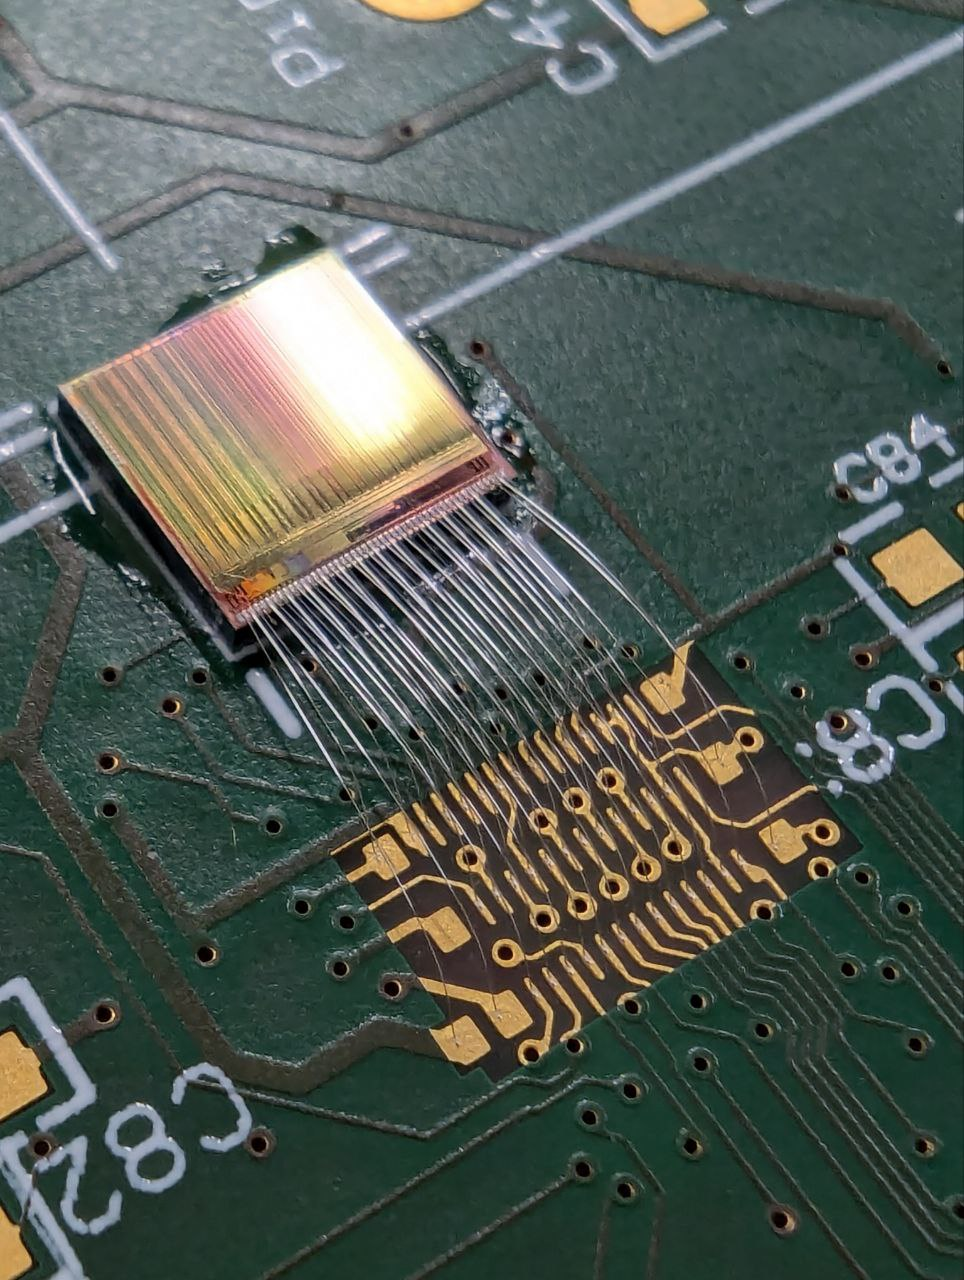
\includegraphics[width=\linewidth,height=0.62\textheight,keepaspectratio]{images/die-on-board.jpg}\\[0.2em]
      {\scriptsize\color{cobgrey} A bare die on a test PCB, wires fanning out to the bond fingers.}
  \end{columns}
\end{frame}

% ======================================================================
% 2. Different ways to bond
\begin{frame}{Different ways to connect die and board}
  \small
  \begin{columns}[T]
    \column{0.49\textwidth}
      \centering
      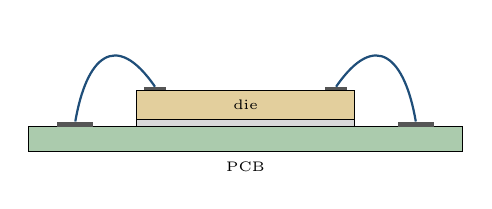
\begin{tikzpicture}[scale=0.92]
        \draw[fill=cobgreen!40] (0,0) rectangle (6,0.35);
        \fill[cobgrey] (0.4,0.35) rectangle (0.9,0.42); \fill[cobgrey] (5.1,0.35) rectangle (5.6,0.42);
        \draw[fill=black!15] (1.5,0.35) rectangle (4.5,0.45);
        \draw[fill=cobgold!40] (1.5,0.45) rectangle (4.5,0.85);
        \fill[cobgrey] (1.6,0.85) rectangle (1.9,0.9); \fill[cobgrey] (4.1,0.85) rectangle (4.4,0.9);
        \draw[thick, cobblue] (1.75,0.9) .. controls (1.2,1.7) and (0.8,1.3) .. (0.65,0.42);
        \draw[thick, cobblue] (4.25,0.9) .. controls (4.8,1.7) and (5.2,1.3) .. (5.35,0.42);
        \node[font=\tiny] at (3,0.65) {die};
        \node[font=\tiny, anchor=north] at (3,0.0) {PCB};
      \end{tikzpicture}\\[0.1em]
      \textbf{Wire bonding}: die glued first, then thin wires from die pads to board pads (wedge or ball)\\[1.2em]
      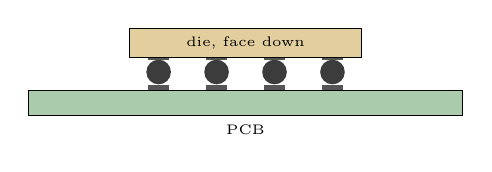
\begin{tikzpicture}[scale=0.92]
        \draw[fill=cobgreen!40] (0,0) rectangle (6,0.35);
        \foreach \x in {1.8,2.6,3.4,4.2} {
          \fill[cobgrey] (\x-0.15,0.35) rectangle (\x+0.15,0.42);
          \fill[cobgrey!70!black] (\x,0.6) circle (0.17);
          \fill[cobgrey] (\x-0.15,0.77) rectangle (\x+0.15,0.8);
        }
        \draw[fill=cobgold!40] (1.4,0.8) rectangle (4.6,1.2);
        \node[font=\tiny] at (3,1.0) {die, face down};
        \node[font=\tiny, anchor=north] at (3,0.0) {PCB};
      \end{tikzpicture}\\[0.1em]
      \textbf{Flip-chip}: die face down, bumps touch the board pads, no wires
    \column{0.49\textwidth}
      \centering
      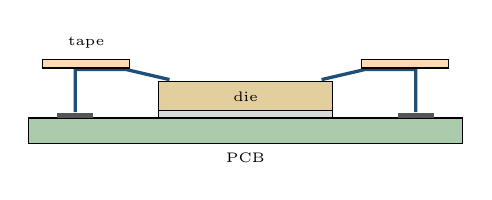
\begin{tikzpicture}[scale=0.92]
        \draw[fill=cobgreen!40] (0,0) rectangle (6,0.35);
        \fill[cobgrey] (0.4,0.35) rectangle (0.9,0.42); \fill[cobgrey] (5.1,0.35) rectangle (5.6,0.42);
        \draw[fill=black!15] (1.8,0.35) rectangle (4.2,0.45);
        \draw[fill=cobgold!40] (1.8,0.45) rectangle (4.2,0.85);
        \draw[very thick, cobblue] (1.95,0.88) -- (1.35,1.02) -- (0.65,1.02) -- (0.65,0.43);
        \draw[very thick, cobblue] (4.05,0.88) -- (4.65,1.02) -- (5.35,1.02) -- (5.35,0.43);
        \draw[fill=orange!30] (0.2,1.04) rectangle (1.4,1.16);
        \draw[fill=orange!30] (4.6,1.04) rectangle (5.8,1.16);
        \node[font=\tiny] at (3,0.65) {die};
        \node[font=\tiny, anchor=south] at (0.8,1.18) {tape};
        \node[font=\tiny, anchor=north] at (3,0.0) {PCB};
      \end{tikzpicture}\\[0.1em]
      \textbf{TAB} (tape automated bonding): metal leads on a flexible tape connect die and board\\[1.2em]
      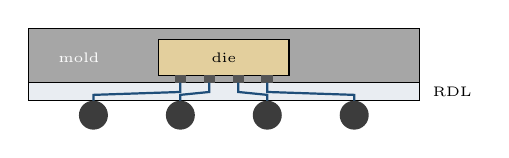
\begin{tikzpicture}[scale=0.92]
        \draw[fill=black!35] (0.3,0.85) rectangle (5.7,1.6);
        \draw[fill=cobgold!40] (2.1,0.95) rectangle (3.9,1.45);
        \draw[fill=cobblue!10] (0.3,0.6) rectangle (5.7,0.85);
        \foreach \x/\b in {2.4/1.2, 2.8/2.4, 3.2/3.6, 3.6/4.8} {
          \fill[cobgrey] (\x-0.08,0.85) rectangle (\x+0.08,0.95);
          \draw[cobblue, thick] (\x,0.85) -- (\x,0.72) -- (\b,0.68) -- (\b,0.58);
          \fill[cobgrey!70!black] (\b,0.4) circle (0.2);
        }
        \node[font=\tiny, color=white] at (1.0,1.2) {mold};
        \node[font=\tiny] at (3,1.2) {die};
        \node[font=\tiny, anchor=west] at (5.75,0.72) {RDL};
      \end{tikzpicture}\\[0.1em]
      \textbf{FOPLP}: dies in a panel, redistribution layers fan the pads out to solder balls
  \end{columns}
  \vfill
  \centering\footnotesize\color{cobgrey}
  Wire bonding is the one a lab or a hackerspace can actually do:
  a used manual bonder starts around \$25k, a new CNC bonder above \$150k.
\end{frame}

% ======================================================================
% 3. Wire bonding
\begin{frame}{Wire bonding: an ultrasonic weld at room temperature}
  \begin{columns}[T]
    \column{0.56\textwidth}
      \footnotesize
      Tool presses an Al, Au or Cu wire onto the pad and vibrates it (60--140\,kHz).
      Oxides break, clean metal meets clean metal, the atoms interdiffuse.
      \vspace{0.4em}

      \centering
      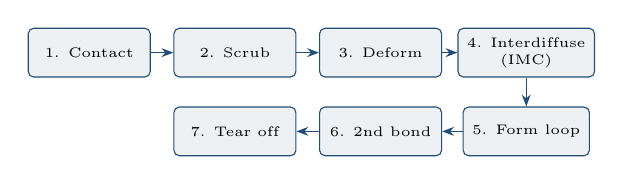
\begin{tikzpicture}[
          bstep/.style={draw=cobblue, fill=cobblue!8, rounded corners=2pt,
                       minimum width=1.55cm, minimum height=0.62cm, font=\tiny, align=center},
          arr/.style={-{Stealth[length=1.5mm]}, cobblue}]
        \node[bstep] (a) at (0,0)    {1. Contact};
        \node[bstep] (b) at (1.85,0) {2. Scrub};
        \node[bstep] (c) at (3.7,0)  {3. Deform};
        \node[bstep] (d) at (5.55,0) {4. Interdiffuse\\(IMC)};
        \node[bstep] (e) at (5.55,-1.0) {5. Form loop};
        \node[bstep] (f) at (3.7,-1.0)  {6. 2nd bond};
        \node[bstep] (g) at (1.85,-1.0) {7. Tear off};
        \draw[arr] (a)--(b); \draw[arr] (b)--(c); \draw[arr] (c)--(d);
        \draw[arr] (d)--(e); \draw[arr] (e)--(f); \draw[arr] (f)--(g);
      \end{tikzpicture}
      \vspace{0.5em}

      \scriptsize
      \begin{tabular}{@{}lL{2.4cm}L{2.6cm}@{}}
        \toprule
        \textbf{Parameter} & \textbf{Too low} & \textbf{Too high}\\
        \midrule
        Bond force       & Non-stick on pad (NSOP) & Cratering, pad damage\\
        Ultrasonic power & Poor scrubbing, NSOP    & Wire necking, cratering\\
        Bond time        & Bond lift               & Brittle IMCs, pad damage\\
        Cleanliness      & NSOP, bond lift         & -- no drawback\\
        \bottomrule
      \end{tabular}
    \column{0.40\textwidth}
      \centering
      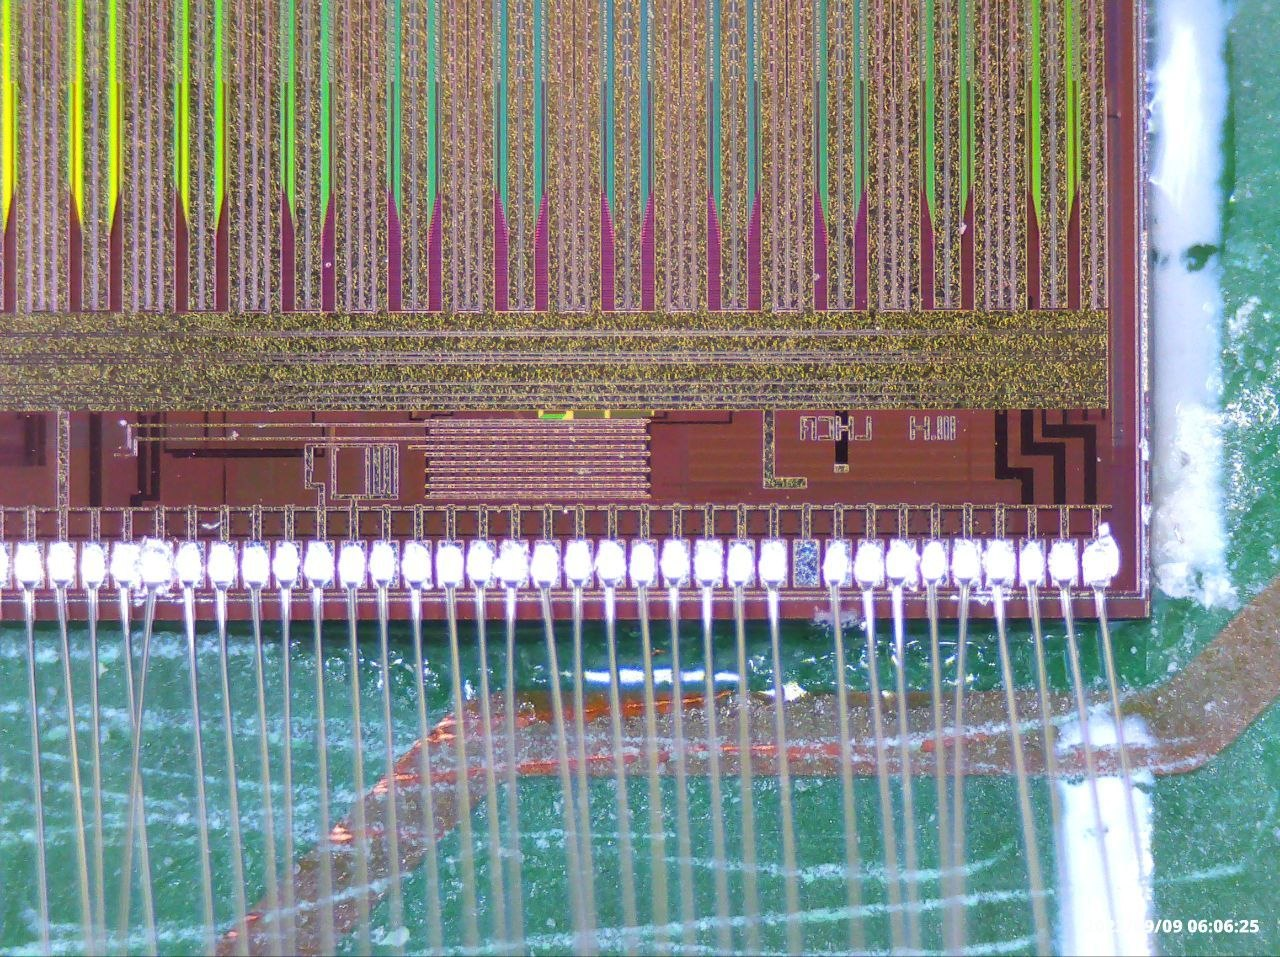
\includegraphics[width=\linewidth]{images/bond-wires-on-pads.jpg}\\[0.2em]
      {\scriptsize\color{cobgrey} Aluminium wedge bonds on the pad row of a pixel readout chip.}\\[0.6em]
      {\scriptsize\color{cobgrey} Full details: \textit{Poor Man's Introduction to Wire-Bonding},
      KiCon Europe 2025 / KiCon Asia 2025.}
  \end{columns}
\end{frame}

% ======================================================================
% 4. TAB bonding
\begin{frame}{TAB: glue the die, connect it with a flex}
  \footnotesize
  \begin{columns}[T]
    \column{0.5\textwidth}
      \begin{block}{Tape automated bonding}
        \begin{itemize}\setlength\itemsep{0.05em}
          \item Copper leads on a flexible tape (or a flex PCB)
          \item All leads of a die are connected \textbf{in one step}, not wire by wire
          \item No loops: low inductance, low profile
          \item The lead pattern is defined once, by the flex design
        \end{itemize}
      \end{block}
      \begin{alertblock}{The catch: tolerances}
        Wires are placed one by one, so each wire follows the die where it really sits.
        A flex has a \textbf{fixed pattern}: if the die shifts during placement,
        \textbf{every contact} misses at once.
      \end{alertblock}
    \column{0.46\textwidth}
      \centering
      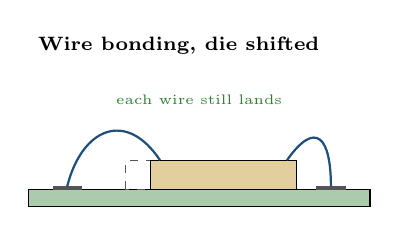
\begin{tikzpicture}[scale=0.62]
        % wire bonding: shifted die, wires still land
        \node[font=\scriptsize\bfseries, anchor=west] at (0,3.3) {Wire bonding, die shifted};
        \draw[fill=cobgreen!40] (0,0) rectangle (7,0.35);
        \fill[cobgrey] (0.5,0.35) rectangle (1.1,0.42); \fill[cobgrey] (5.9,0.35) rectangle (6.5,0.42);
        \draw[dashed, cobgrey] (2.0,0.35) rectangle (5.0,0.95);
        \draw[fill=cobgold!40] (2.5,0.35) rectangle (5.5,0.95);
        \draw[thick, cobblue] (2.7,0.95) .. controls (2.0,2.0) and (1.1,1.6) .. (0.8,0.42);
        \draw[thick, cobblue] (5.3,0.95) .. controls (5.9,1.8) and (6.2,1.4) .. (6.2,0.42);
        \node[font=\tiny, color=cobgreen] at (3.5,2.2) {each wire still lands};
      \end{tikzpicture}\\[0.8em]
      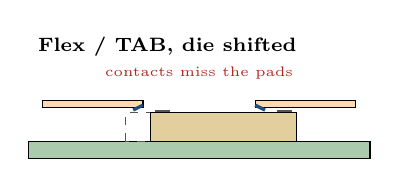
\begin{tikzpicture}[scale=0.62]
        \node[font=\scriptsize\bfseries, anchor=west] at (0,2.3) {Flex / TAB, die shifted};
        \draw[fill=cobgreen!40] (0,0) rectangle (7,0.35);
        \draw[dashed, cobgrey] (2.0,0.35) rectangle (5.0,0.95);
        \draw[fill=cobgold!40] (2.5,0.35) rectangle (5.5,0.95);
        \fill[cobgrey] (2.6,0.95) rectangle (2.9,1.0); \fill[cobgrey] (5.1,0.95) rectangle (5.4,1.0);
        \draw[fill=orange!30] (0.3,1.05) rectangle (2.35,1.2);
        \draw[fill=orange!30] (4.65,1.05) rectangle (6.7,1.2);
        \draw[very thick, cobblue] (2.35,1.1) -- (2.15,1.0);
        \draw[very thick, cobblue] (4.65,1.1) -- (4.85,1.0);
        \node[font=\tiny, color=cobred] at (3.5,1.75) {contacts miss the pads};
      \end{tikzpicture}
      \vfill
      {\scriptsize\color{cobgrey} Open question: which placement tolerance can a flex take?
      To be evaluated experimentally.}
  \end{columns}
\end{frame}

% ======================================================================
% 5. Challenges
\begin{frame}{The challenge is not the bond, it is the board}
  \scriptsize
  \begin{columns}[T]
    \column{0.485\textwidth}
      \begin{alertblock}{1. The data is scattered}
        GDS, schematic, process documents, a slide. The copies drift apart.
      \end{alertblock}
      \begin{alertblock}{2. Chicken and egg}
        Wire length depends on the land pattern you are trying to design.
      \end{alertblock}
      \begin{alertblock}{3. New chip, new footprint}
        Every chip iteration needs its own land pattern, drawn pad by pad.
      \end{alertblock}
      \begin{alertblock}{4. Tolerances stay invisible}
        A die placed 50--100\,$\mu$m off moves every wire landing point.
      \end{alertblock}
    \column{0.485\textwidth}
      \centering
      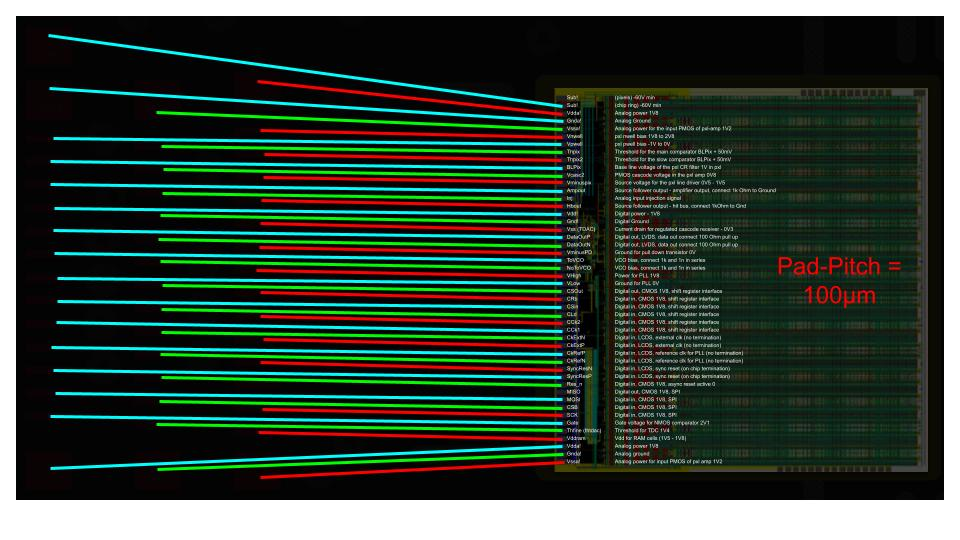
\includegraphics[width=\linewidth]{images/legacy-bonding-plan-example.jpg}\\[0.2em]
      {\scriptsize\color{cobgrey} A typical bonding plan: a die photo, pad names and coloured lines on a slide.
      It works, but no tool can read it.}
  \end{columns}
\end{frame}

% ======================================================================
% 6. open.cob.json
\begin{frame}{open.cob.json: describe the chip once, generate the rest}
  \small
  \begin{columns}[T]
    \column{0.52\textwidth}
      One open JSON file per die, between chip designer and PCB designer:
      \begin{itemize}\setlength\itemsep{0.15em}
        \item \texttt{die}: size, notch, pads (from the GDS)
        \item \texttt{pcb}: pad shapes, pads, cutouts, fiducials
        \item \texttt{wires}: die pad to board pad, material, loop
        \item \texttt{assembly}, \texttt{tolerances}, \texttt{units}, \texttt{meta}
        \item \texttt{"unspecified"} = unknown, \texttt{"none"} = deliberately absent
      \end{itemize}
      \vspace{0.4em}
      \centering
      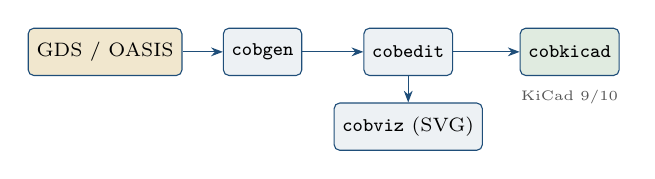
\begin{tikzpicture}[
          box/.style={draw=cobblue, fill=cobblue!8, rounded corners=2pt, font=\scriptsize,
                      minimum height=0.6cm, inner sep=3pt},
          arr/.style={-{Stealth[length=1.5mm]}, cobblue}]
        \node[box, fill=cobgold!20] (gds) at (0,0) {GDS / OASIS};
        \node[box] (gen) at (2.0,0)  {\texttt{cobgen}};
        \node[box] (ed)  at (3.85,0) {\texttt{cobedit}};
        \node[box, fill=cobgreen!15] (ki) at (5.9,0) {\texttt{cobkicad}};
        \node[box] (viz) at (3.85,-0.95) {\texttt{cobviz} (SVG)};
        \draw[arr] (gds)--(gen); \draw[arr] (gen)--(ed); \draw[arr] (ed)--(ki);
        \draw[arr] (ed)--(viz);
        \node[font=\tiny, color=cobgrey, below=0.05cm of ki] {KiCad 9/10};
      \end{tikzpicture}
    \column{0.44\textwidth}
      \centering
      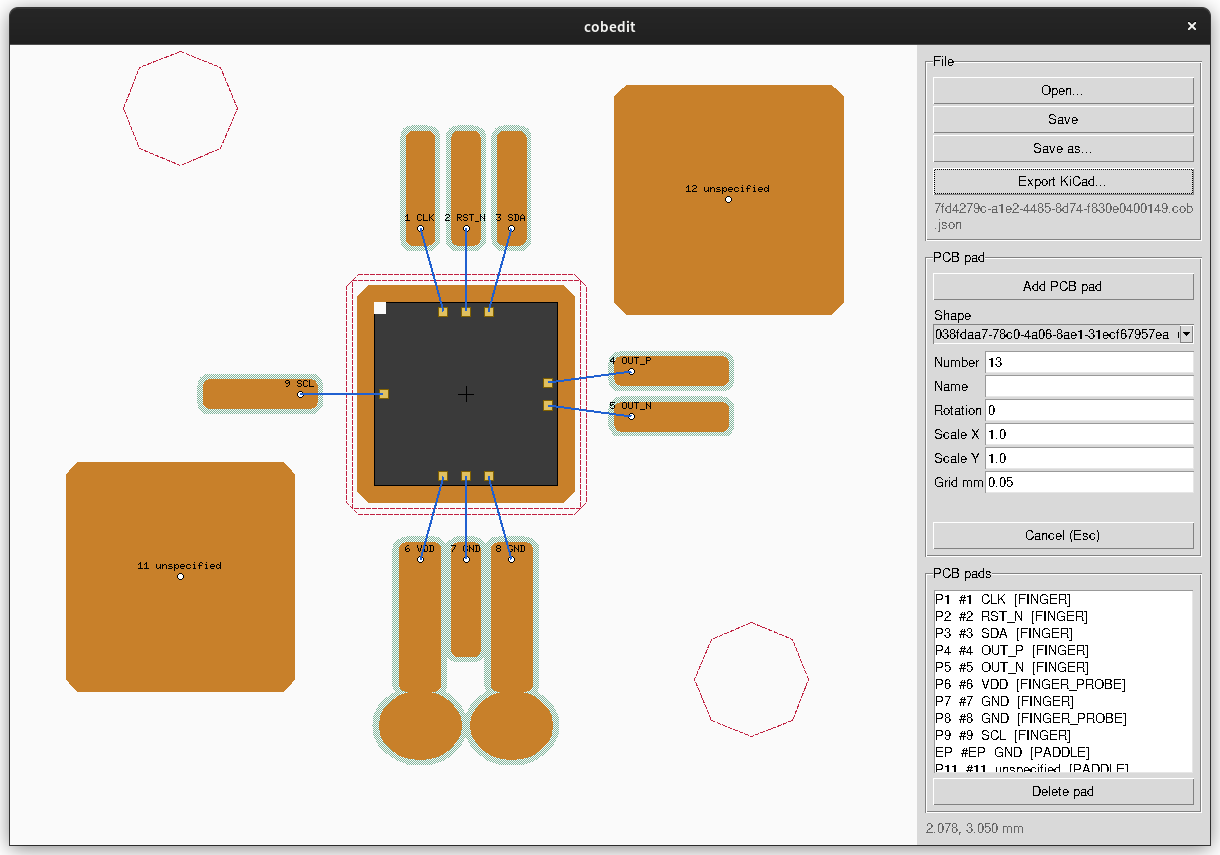
\includegraphics[width=\linewidth]{images/cobedit-screenshot.png}\\[0.3em]
      \raggedright\footnotesize
      Works today with \textbf{gf180mcu} and the wafer.space reticles.\\[0.3em]
      \textbf{Bring your chip and your PDK}: run it through \texttt{cobgen} and tell me what broke.\\[0.4em]
      \scriptsize\color{cobgrey}
      \faGithub\ github.com/MaxClerkwell/open.cob.json\\
      DOI 10.5281/zenodo.22850092 \quad CC BY 4.0
  \end{columns}
\end{frame}

% ======================================================================
\begin{frame}{About me - Stephan Bökelmann}
  \setlength{\stackw}{0.7\textwidth}
  \newcommand{\aboutstack}{%
    \begin{minipage}[t]{\stackw}
      \footnotesize
      \begin{beamercolorbox}[wd=\linewidth,sep=0.4em]{block title example}
        \textbf{Need something special bonded? Hit me up and let's talk about it.}
      \end{beamercolorbox}
      \vspace{0.2em}
      \begin{beamercolorbox}[wd=\linewidth,sep=0.4em]{block title alerted}
        Scientific Research Engineer at Facility for Antiproton and Ion Research
      \end{beamercolorbox}
      \vspace{0.2em}
      \begin{beamercolorbox}[wd=\linewidth,sep=0.4em]{block title alerted}
        \textbf{Hire me and my team via nabla B engineering}
      \end{beamercolorbox}
      \vspace{0.2em}
      \begin{beamercolorbox}[wd=\linewidth,sep=0.4em]{block title alerted}
        \textbf{Follow me} for digital design, physics and ASICs\\[0.3em]
        \scriptsize
        \faGlobe\ maxclerkwell.tech \quad \faInstagram\ Instagram \quad \xhslogo\ Xiaohongshu \quad \faDiscord\ Discord
      \end{beamercolorbox}
    \end{minipage}}
  \sbox{\stackbox}{\aboutstack}
  \setlength{\stackh}{\dimexpr\ht\stackbox+\dp\stackbox\relax}
  \noindent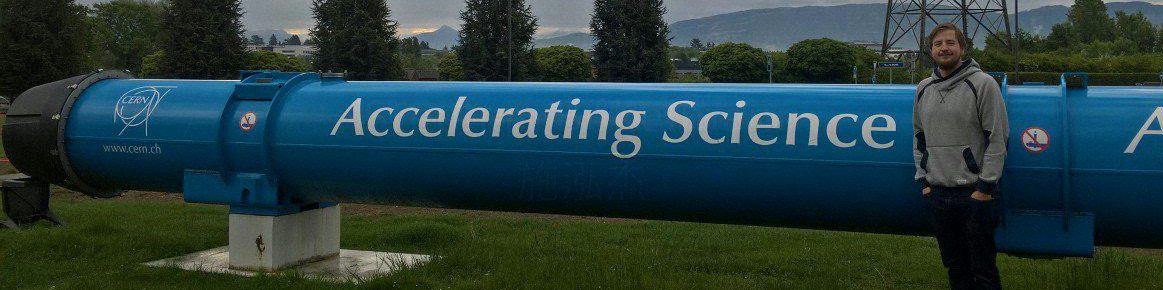
\includegraphics[width=\textwidth]{images/portrait-cern.jpg}
  \vfill
  \begin{columns}[T,onlytextwidth]
    \column{\stackw}
      \aboutstack
    \column{\stackh}
      \qrcode[tight,height=\stackh]{https://nabla-b.engineering/en/business-card/}
  \end{columns}
\end{frame}

% ======================================================================
% Extra / backup slide
\begin{frame}{Extra: Design for Bonding}
  \footnotesize
  \begin{columns}[T]
    \column{0.485\textwidth}
      \begin{block}{On the chip}
        \begin{itemize}\setlength\itemsep{0.2em}
          \item Pad openings large enough for the tool\\
                {\scriptsize\color{cobgrey} e.g.\ $\geq$\,70\,$\mu$m for a 25\,$\mu$m Al wedge}
          \item Pads on the die edge, not in the middle of the die
          \item Top metallization decides wire, force and temperature: clarify it early
          \item Plan ground / substrate pads and extra probe pads
          \item A notch or marker, so the orientation is clear under the microscope
        \end{itemize}
      \end{block}
    \column{0.485\textwidth}
      \begin{block}{On the board}
        \begin{itemize}\setlength\itemsep{0.2em}
          \item Surface finish matching the wire\\
                {\scriptsize\color{cobgrey} e.g.\ Al wedge on ENIG}
          \item Bond finger pitch and angle matching the pads; stagger when tight
          \item Short wires, equal length where it matters (EMC, differential pairs)
          \item Die attach area, via keepout under the die, fiducials
          \item Budget for placement tolerance: 50--100\,$\mu$m
        \end{itemize}
      \end{block}
  \end{columns}
  \vfill
  \begin{center}
    \small Not sure your chip or board fits this? \textbf{Bring it, let's talk.}
  \end{center}
\end{frame}

% ======================================================================
% Extra: the bonder program
\newcommand{\shot}[3]{%
  \begin{minipage}[t]{#1}\centering
    \includegraphics[width=\linewidth,height=3.1cm,keepaspectratio]{images/#2}\\[0.2em]
    {\scriptsize\textbf{#3}}
  \end{minipage}}
\begin{frame}{Extra: what a bonder program looks like}
  \footnotesize
  Every wire on the bonder needs its own set of parameters:\\[0.6em]
  \centering
  \shot{0.27\textwidth}{bonder-placement.jpg}{1. Placement}\hfill
  \shot{0.27\textwidth}{bonder-bond-params.jpg}{2. Bond: force, US, time}\hfill
  \shot{0.17\textwidth}{bonder-loop-params.jpg}{3. Loop trajectory}\hfill
  \shot{0.27\textwidth}{bonder-tear-params.jpg}{4. Tear off}
  \vfill
  \raggedright
  \begin{itemize}\setlength\itemsep{0.1em}
    \item Placement comes from chip and board; bond and loop from wire, metallization and wire length
    \item All of this is already in a \texttt{*.cob.json} file
    \item \textbf{Next step for open.cob.json: generate the bonder program directly from the file}
  \end{itemize}
\end{frame}

% ======================================================================
% Extra: from the lab
\newcommand{\labpic}[2]{%
  \begin{minipage}[t]{0.235\textwidth}\centering
    \includegraphics[width=\linewidth,height=0.6\textheight,keepaspectratio]{images/#1}\\[0.2em]
    {\scriptsize\color{cobgrey} #2}
  \end{minipage}}
\begin{frame}{Extra: from the lab}
  \centering
  \labpic{lab-die-on-pcb.jpg}{Bare die glued and bonded on a test PCB}\hfill
  \labpic{lab-pixel-chip-microscope.jpg}{Bonded pixel chip under the microscope}\hfill
  \labpic{lab-eyepiece.jpg}{What the bonder operator sees}\hfill
  \labpic{lab-cleanroom.jpg}{Cleanroom, mask on}
  \vfill
  \small Two years of hands-on bonding of HV-MAPS detector chips.
  \textbf{Need something special bonded? Let's talk.}
\end{frame}

\end{document}
